\documentclass{article}

%Header Dimensions
%https://tex.stackexchange.com/questions/40183/problem-with-the-header-footer-width#40184
\usepackage[margin=0.5in,bottom=0.5in,top=0.5in]{geometry}

%Package required for empty set
\usepackage{amssymb}

%Package required for Comb/Perm symbol and matrices
\usepackage{amsmath}

%Package for graphics
\usepackage{graphicx}

%Package for placing graphics
\usepackage{float}

%Places box around graphics
% Uncomment to box 
% \floatstyle{boxed} 
% \restylefloat{figure}


%For inserting code
\usepackage{listings}
%https://www.sharelatex.com/learn/Code_listing

\begin{document}

	
%%%%%%%%%%%%%%%%%
%CUSTOM COMMANDS%
%%%%%%%%%%%%%%%%%

	%This line surpresses the page number
%https://tex.stackexchange.com/questions/7355/how-to-suppress-page-number
\thispagestyle{empty}

%Make empty set pretty
% https://tex.stackexchange.com/questions/22798/nice-looking-empty-setup
\let\oldemptyset\emptyset
\let\emptyset\varnothing


%Combinatorial notation
%From https://tex.stackexchange.com/questions/107125/is-there-a-command-to-write-the-form-of-a-combination-or-permutation
\newcommand*{\Perm}[2]{{}^{#1}\!P_{#2}}
\newcommand*{\Comb}[2]{{}_{#1}C_{#2}}


	
\textbf{	Matt Fletcher CS317-02 Homework 1}
\smallskip


1.  


\begin{figure}[H]
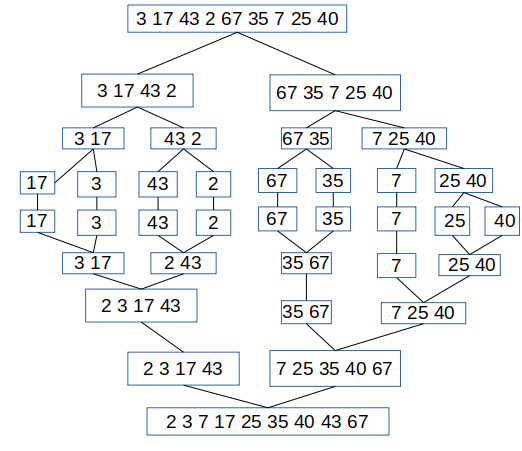
\includegraphics[scale=0.5]{./P1/sorted}
\centering
\end{figure}


\noindent\rule{8cm}{0.4pt}



2. 

Three steps:

a) Move R to left, and L to R until $R<P$ and $L>P$. 

b) If during (a) R and L did not cross, swap R and L, and continue (a). 

c). If during (a) R and L did cross, swap R and P, freeze P in its new place, split the list in 2 around P, and recursively continue (a) on each new list. 

An asterisk next to an element indicates that it is frozen. 

\begin{lstlisting}
P 	L 							R
43	21	90	8	44	35	6	2	13

P 		L 						R
43	21	90	8	44	35	6	2	13

P 		R 						L
43	21	13	8	44	35	6	2	90

P 		L 						R
43	21	13	8	44	35	6	2	90

P 		 		L			R	
43	21	13	8	44	35	6	2	90

P 		 		L			R	
43	21	13	8	2	35	6	44	90

P 		 				R	L	
43	21	13	8	2	35	6	44	90

R 		 				P	L	
6	21	13	8	2	35	43	44	90

P	L	 			R		PL	R
6	21	13	8	2	35	43*	44	90

P	L	 		R			PR	L
6	21	13	8	2	35	43*	44	90

P	R	L 						
6	2	13	8	21	35	43*	44*	90

		P 	L		R			
2	6*	13	8	21	35	43*	44*	90

		P 	R	L				
2	6*	13	8	21	35	43*	44*	90

		 		PL	R			
2	6*	8	13*	21	35	43*	44*	90

		 		PR	L			
2	6*	8	13*	21	35	43*	44*	90

		 						
2	6*	8	13*	21*	35	43*	44*	90

\end{lstlisting}

All elements are either frozen or single element lists, therefore, the list is sorted. 

\noindent\rule{8cm}{0.4pt}

3. 

Five applications of graph theory: social media connections, navigation, cellular connections to towers, circuit design, register allocation

\noindent\rule{8cm}{0.4pt}


4. 
A directed graph has edges which indicate the direction they travel. The direction of travel cannot oppose the node. On the other hand, an undirected graph allows travel both ways along any edge. 

\noindent\rule{8cm}{0.4pt}

5. 

a) Edges: ac, cf, ab, be, bd
	
	Nodes:a,b,c,d,e,f

b) Edges: fc, ca, ba, be, bd
	
	Nodes:  a,c,f,b,e,d


\noindent\rule{8cm}{0.4pt}

6. 

a) Adjacency List

\begin{lstlisting}
[ a ]-->[ b ]-->[ c ]-->[ d ]-->[ e ]-->[ f ]-->[ g ]
 |       |       |       |       |       |       | 
 v       v       v       v       v       v       v
[->b]   [->d]   [->f]   [->b]   [->b]   [->c]   [->e]
 |       |       |       |       |       |       | 
 v       v       v       v       v       v       v
[->c]   [->e]   [->a]   [->0]   [->g]   [->g]   [->f]
 |       |       |               |       |       | 
 v       v       v               v       v       v
[->0]   [->a]   [->0]           [->0]   [->0]   [->0]
         |
         v
        [->0] 
\end{lstlisting}


a) Adjacency Matrix

\begin{table}[H]
\begin{tabular}{l|l|l|l|l|l|l|l|}
\cline{2-8}
 & A & B & C & D & E & F & G \\ \hline
\multicolumn{1}{|l|}{A} & 0 & 1 & 1 & 0 & 0 & 0 & 0 \\ \hline
\multicolumn{1}{|l|}{B} & 1 & 0 & 0 & 1 & 1 & 0 & 0 \\ \hline
\multicolumn{1}{|l|}{C} & 1 & 0 & 0 & 0 & 0 & 1 & 0 \\ \hline
\multicolumn{1}{|l|}{D} & 0 & 1 & 0 & 0 & 0 & 0 & 0 \\ \hline
\multicolumn{1}{|l|}{E} & 0 & 1 & 0 & 0 & 0 & 0 & 1 \\ \hline
\multicolumn{1}{|l|}{F} & 0 & 0 & 1 & 0 & 0 & 0 & 1 \\ \hline
\multicolumn{1}{|l|}{G} & 0 & 0 & 0 & 0 & 1 & 1 & 0 \\ \hline
\end{tabular}
\end{table}


b) Adjacency List

\begin{lstlisting}
[ a ]-->[ b ]-->[ c ]-->[ d ]-->[ e ]-->[ f ]-->[ g ]
 |       |       |       |       |       |       | 
 v       v       v       v       v       v       v
[->b]   [->d]   [->a]   [->0]   [->0]   [->c]   [->0]
 |       |       |                       |     
 v       v       v                       v    
[->g]   [->e]   [->0]                   [->g]
 |       |                               |  
 v       v                               v   
[->0]   [->0]                           [->0]

\end{lstlisting}

b) Adjacency Matrix

\begin{table}[H]
\begin{tabular}{l|l|l|l|l|l|l|l|}
\cline{2-8}
 & A & B & C & D & E & F & G \\ \hline
\multicolumn{1}{|l|}{A} & 0 & 1 & 0 & 0 & 0 & 0 & 1 \\ \hline
\multicolumn{1}{|l|}{B} & 0 & 0 & 0 & 1 & 1 & 0 & 0 \\ \hline
\multicolumn{1}{|l|}{C} & 1 & 0 & 0 & 0 & 0 & 0 & 0 \\ \hline
\multicolumn{1}{|l|}{D} & 0 & 0 & 0 & 0 & 0 & 0 & 0 \\ \hline
\multicolumn{1}{|l|}{E} & 0 & 0 & 0 & 0 & 0 & 0 & 0 \\ \hline
\multicolumn{1}{|l|}{F} & 0 & 0 & 1 & 0 & 0 & 0 & 1 \\ \hline
\multicolumn{1}{|l|}{G} & 0 & 0 & 0 & 0 & 0 & 0 & 0 \\ \hline
\end{tabular}
\end{table}

\noindent\rule{8cm}{0.4pt}


7.  Traversal order:

A 1/16

B 2/9

C 10/15

D 3/4

E 5/8

F 11/14

G 12/13

Stack order:

Top $\rightarrow$$\rightarrow$$\rightarrow$ $\rightarrow$Bottom

$\boxed{G F C H E D B A}$

\noindent\rule{8cm}{0.4pt}


8.  Traversal order:

A 1

B 2

C 2

D 3

E 3 

F 4

G 5

Queue:

Front $\rightarrow$$\rightarrow$$\rightarrow$ $\rightarrow$Back

$\boxed{A B C D E F G}$

\noindent\rule{8cm}{0.4pt}


9.  

Efficiency of Matrix: $\Theta(\|V^2\|)$

Efficiency of List: $\Theta(\|V\|+  \|E\|)$

\noindent\rule{8cm}{0.4pt}


10. The greedy technique builds a solution piece by piece by picking the most obvious benefit first, without ever reconsidering a decision. It generates a globally optimal solution from a locally optimized choice. 

The greedy algorithm works when subproblems are perfect subsets without overlap of a larger problem. 

For example, in the change making problem done in class:

If the coin values are 1,5,10,25,50, a greedy algorithm WILL work in this case. This is because there is no coin value that cannot be made by a combination of smaller coins. 


However, if the coin values are 1,5,10,15,25,50, a greedy algorithm will not find the optimal solution. This is because some combinations of smaller coins could make a more optimal solution than larger coins. 

The greedy choice property: Generating a globally optimal solution from a locally optimized choice. 




\noindent\rule{8cm}{0.4pt}

11. A spanning tree is a set of edges that connects every node in the graph without forming loops or cycles. 


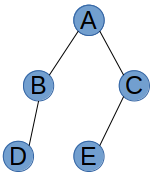
\includegraphics[scale=0.5]{./P11/1}
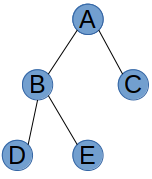
\includegraphics[scale=0.5]{./P11/2}
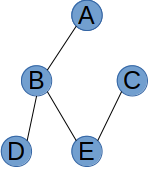
\includegraphics[scale=0.5]{./P11/3}
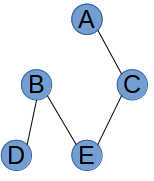
\includegraphics[scale=0.5]{./P11/4}
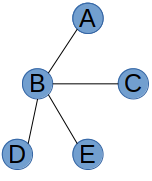
\includegraphics[scale=0.5]{./P11/5}
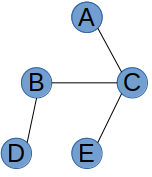
\includegraphics[scale=0.5]{./P11/6}
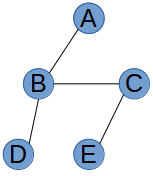
\includegraphics[scale=0.5]{./P11/7}

I'm pretty sure I found all of them, however, I might be missing one. 

\noindent\rule{8cm}{0.4pt}

12. A minimum spanning tree (MST) is the smallest tree that connects every node in the graph. If the graph is weighted, the smallest tree has the smallest sum of weights. If the graph is unweighted, the MST has the smallest number of edges. 

An example of a minimum spanning tree is determining the minimum amount of wire needed to connect multiple nodes. 

\noindent\rule{8cm}{0.4pt}

13. 

Kruskal's Algorithm: 

$\rightarrow$1. Create a table with each edge sorted in ascending order. 
\begin{table}[H]
\begin{tabular}{|l|l|l|l|l|l|l|l|l|l|l|}
\hline
Edge & CD & DE & AD & AE & BC & AB & BE & BD & AC & BC \\ \hline
Weight & 1 & 2 & 3 & 4 & 5 & 6 & 6 & 8 & 9 & 11 \\ \hline
\end{tabular}
\end{table}


$\rightarrow$2. Starting from either node on the smallest line, attach the next smallest line that does not create a loop. 

Start by attaching line $CD$, weight 1. 

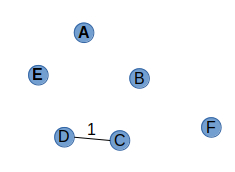
\includegraphics[scale=0.5]{./P13/kruskals/1}

Then, find the smallest weighted edge from any end node that does not create a cycle. This is edge DE. 

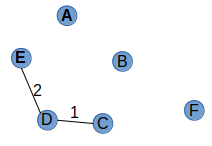
\includegraphics[scale=0.5]{./P13/kruskals/2}

Same as before, add edge AD. 

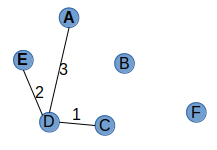
\includegraphics[scale=0.5]{./P13/kruskals/3}

Although AE is the next smallest edge, adding it would create a cycle. So we add BC instead. 

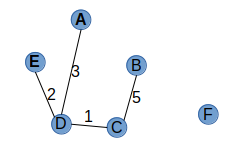
\includegraphics[scale=0.5]{./P13/kruskals/4}

Add the next edge. 

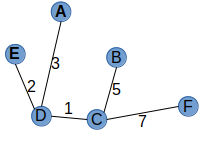
\includegraphics[scale=0.5]{./P13/kruskals/5}

At this point, all the nodes are connected and adding any more lines would result in a cycle being created. Hence, we are done. 



Prims algorithm starts from some vertex (Vertex A in this example) and finds the smallest addition that can be added to the current tree in order to not create a cycle. 

A dashed line indicated that edge has been selected. 

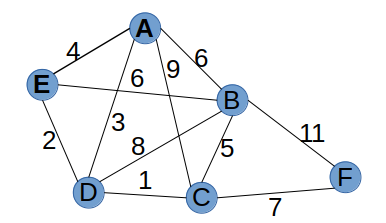
\includegraphics[scale=0.5]{./P13/prims/0}

Start at vertex A. There are 4 edges that can be selected: AE, AD, AC, and AB. AE has the lowest weight, so we select that edge. 

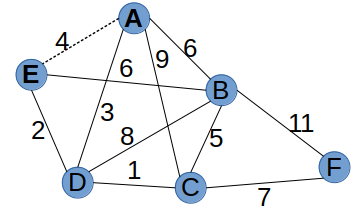
\includegraphics[scale=0.5]{./P13/prims/1}

Now, we check all of the edges coming out of both vertex A and E. The lowest weight gets selected, and we choose edge ED. 

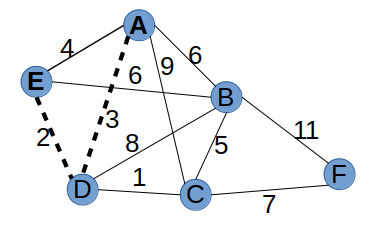
\includegraphics[scale=0.5]{./P13/prims/2}

At this point, we check vertices A, E, and D. Although DA has the lowest weight, it would cause a cycle. So, we skip it and check the other edges. 

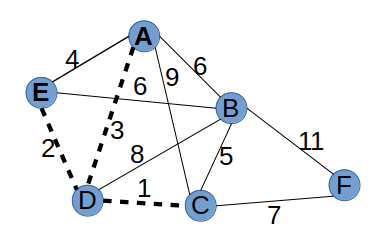
\includegraphics[scale=0.5]{./P13/prims/3}

Continuing...

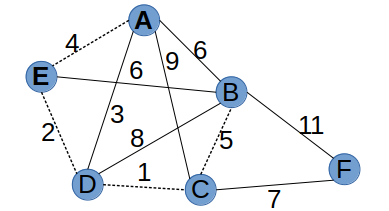
\includegraphics[scale=0.5]{./P13/prims/4}

Almost there...


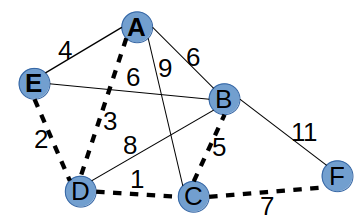
\includegraphics[scale=0.5]{./P13/prims/5}

And done!




We are done because all vertices have been reached, and no loops or cycles have been created. The total weight is $3+2+1+5+7=\boxed{18}$.






\noindent\rule{8cm}{0.4pt}

14. 

Start at vertex A. Find the shortest path to all other vertices, and indicate in table. Use $\infty$ if there is no path. 


\begin{table}[H]
\begin{tabular}{|l|l|l|l|l|l|l|l|}
\hline
V & \textbf{A} & B & C & D & E & F & G \\ \hline
A & $0_A$ & $7_A$ & $3_A$ & $4_DA$ & $\infty$ & $\infty$ & $\infty$ \\ \hline
\end{tabular}
\end{table}

C is the next unvisited vertex to visit having the smallest tentative distance. Therefore, we visit C and check if there exists a shorter path between A and immediate neighbors of C through C. 



\begin{table}[H]
\begin{tabular}{|l|l|l|l|l|l|l|l|}
\hline
V & \textbf{A} & B & \textbf{C} & D & E & F & G \\ \hline
A & $0_A$ & $7_A$ & $3_A$ & $4_D$ & $\infty$ & $\infty_A$ & $\infty_A$ \\ \hline
C & $0_A$ & $7_A$ & $3_A$ & $4_D$ & $12_C$ & $\infty_A$ & $\infty_A$ \\ \hline
\end{tabular}
\end{table}

Now, check B and see if any paths can be optimized or created. A route to F is possible through B, so we change the value from $\infty$ to $10_B$. 

\begin{table}[H]
\begin{tabular}{|l|l|l|l|l|l|l|l|}
\hline
V & \textbf{A} & \textbf{B} & \textbf{C} & D & E & F & G \\ \hline
A & $0_A$ & $7_A$ & $3_A$ & $4_D$ & $\infty$ & $\infty_A$ & $\infty_A$ \\ \hline
C & $0_A$ & $7_A$ & $3_A$ & $4_D$ & $12_C$ & $\infty$ & $\infty_A$ \\ \hline
B & $0_A$ & $7_A$ & $3_A$ & $4_D$ & $12_C$ & $10_B$ & $\infty_A$ \\ \hline
\end{tabular}
\end{table}

D is the next unvisited node. A route through from A to E through D is now shorter than the current route of A to E through D, therefore, we replace the value. 

\begin{table}[H]
\begin{tabular}{|l|l|l|l|l|l|l|l|}
\hline
V & \textbf{A} & \textbf{B} & \textbf{C} & \textbf{D} & E & F & G \\ \hline
A & $0_A$ & $7_A$ & $3_A$ & $4_D$ & $\infty$ & $\infty_A$ & $\infty_A$ \\ \hline
C & $0_A$ & $7_A$ & $3_A$ & $4_D$ & $12_C$ & $\infty$ & $\infty_A$ \\ \hline
B & $0_A$ & $7_A$ & $3_A$ & $4_D$ & $12_C$ & $10_B$ & $\infty_A$ \\ \hline
D & $0_A$ & $7_A$ & $3_A$ & $4_D$ & $6_D$ & $10_B$ & $14_D$ \\ \hline
\end{tabular}
\end{table}

Next, we visit E. No routes are optimized or created during this visit. 

\begin{table}[H]
\begin{tabular}{|l|l|l|l|l|l|l|l|}
\hline
V & \textbf{A} & \textbf{B} & \textbf{C} & \textbf{D} & \textbf{E} & F & G \\ \hline
A & $0_A$ & $7_A$ & $3_A$ & $4_D$ & $\infty$ & $\infty_A$ & $\infty_A$ \\ \hline
C & $0_A$ & $7_A$ & $3_A$ & $4_D$ & $12_C$ & $\infty$ & $\infty_A$ \\ \hline
B & $0_A$ & $7_A$ & $3_A$ & $4_D$ & $12_C$ & $10_B$ & $\infty_A$ \\ \hline
D & $0_A$ & $7_A$ & $3_A$ & $4_D$ & $6_D$ & $10_B$ & $14_D$ \\ \hline
E & $0_A$ & $7_A$ & $3_A$ & $4_D$ & $6_D$ & $10_B$ & $14_D$ \\ \hline
\end{tabular}
\end{table}

Visit F, no routes optimized. Visit G, no routes optimized. Therefore, the table is finished as follows:

\begin{table}[H]
\begin{tabular}{|l|l|l|l|l|l|l|l|}
\hline
V & \textbf{A} & \textbf{B} & \textbf{C} & \textbf{D} & \textbf{E} & \textbf{F} & \textbf{G} \\ \hline
A & $0_A$ & $7_A$ & $3_A$ & $4_D$ & $\infty$ & $\infty_A$ & $\infty_A$ \\ \hline
C & $0_A$ & $7_A$ & $3_A$ & $4_D$ & $12_C$ & $\infty$ & $\infty_A$ \\ \hline
B & $0_A$ & $7_A$ & $3_A$ & $4_D$ & $12_C$ & $10_B$ & $\infty_A$ \\ \hline
D & $0_A$ & $7_A$ & $3_A$ & $4_D$ & $6_D$ & $10_B$ & $14_D$ \\ \hline
E & $0_A$ & $7_A$ & $3_A$ & $4_D$ & $6_D$ & $10_B$ & $14_D$ \\ \hline
F & $0_A$ & $7_A$ & $3_A$ & $4_D$ & $6_D$ & $10_B$ & $14_D$ \\ \hline
G & $0_A$ & $7_A$ & $3_A$ & $4_D$ & $6_D$ & $10_B$ & $14_D$ \\ \hline
\end{tabular}
\end{table}


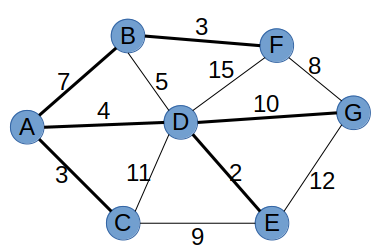
\includegraphics[scale=0.5]{./P14/final}






\noindent\rule{8cm}{0.4pt}


15.  

Create a table of the numbers and their count:

\begin{table}[H]
\begin{tabular}{|l|l|l|l|}
\hline
T & N & S & E \\ \hline
1 & 2 & 2 & 4 \\ \hline
\end{tabular}
\end{table}

Insert these into a priority queue: 

\begin{figure}[H]
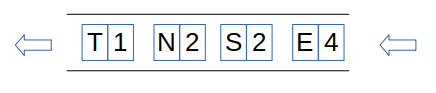
\includegraphics[scale=0.5]{./P15/0}
\centering
\end{figure}

Dequeue the first 2 elements T and N, combine into binary tree:

\begin{figure}[H]
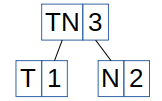
\includegraphics[scale=0.5]{./P15/TN}
\centering
\end{figure}

Queue the newly created element into the queue in its proper position. . 

\begin{figure}[H]
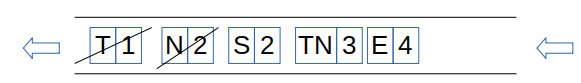
\includegraphics[scale=0.5]{./P15/TN_Queue}
\centering
\end{figure}


Dequeue the next 2 elements, place into binary tree, and queue the newly created element. 


\begin{figure}[H]
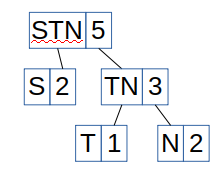
\includegraphics[scale=0.5]{./P15/STN}
\centering
\end{figure}

\begin{figure}[H]
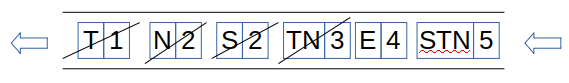
\includegraphics[scale=0.5]{./P15/STN_Queue}
\centering
\end{figure}


Now, dequeue the 2 elements left in the queue, and insert these into a binary tree. 

\begin{figure}[H]
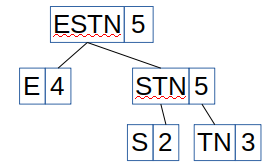
\includegraphics[scale=0.5]{./P15/ESTN}
\centering
\end{figure}

Now, we assign a value to each node. To the left is 0, to the right is 1. 


\begin{figure}[H]
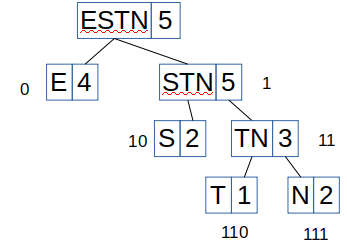
\includegraphics[scale=0.5]{./P15/Scored}
\centering
\end{figure}

According to this, E gets replaced with a 0, S with a 10, T with a 110, and N with a 111. 

Therefore, TENNESSEE gets converted to 110 0 111 111 0 10 10 0 0. 

This is 17 bits, compared to the original 9 8 bit ASCII characters equaling 72 bits. 



\noindent\rule{8cm}{0.4pt}

16. 

Begin by creating a heap. 

Array: 9,4,1,6,3,8,2,10

Take the first element, put it as the root. 
\begin{figure}[H]
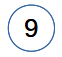
\includegraphics[scale=0.5]{./P16/0}
\centering
\end{figure}

Take the next element, and attach it to the bottom left. No reheaping necessary, because $4<9$. 

\begin{figure}[H]
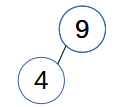
\includegraphics[scale=0.5]{./P16/1}
\centering
\end{figure}

Add the next element to the bottom right. No reheaping necessary. 

\begin{figure}[H]
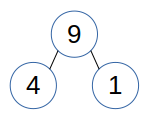
\includegraphics[scale=0.5]{./P16/2}
\centering
\end{figure}


Add the next element to the bottom left of $4$. Because $6>4$, a reheaping is necessary. 

\begin{figure}[H]
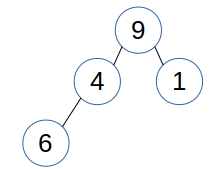
\includegraphics[scale=0.5]{./P16/3}
\centering
\end{figure}


Reheaped. 

\begin{figure}[H]
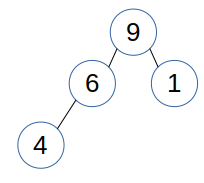
\includegraphics[scale=0.5]{./P16/4}
\centering
\end{figure}


Continue this algorithm until all elements have been added to the list (some steps omitted for clarity.)

\begin{figure}[H]
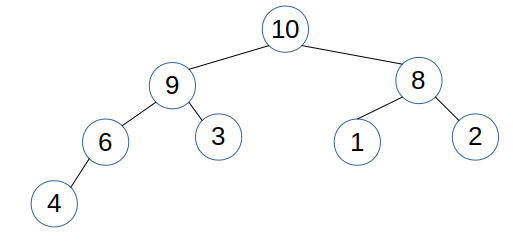
\includegraphics[scale=0.5]{./P16/0full}
\centering
\end{figure}

Now, swap the root element (the max, 10) with the bottom right element (2), and delete the max element. This max element is the largest in the list. 

\begin{figure}[H]
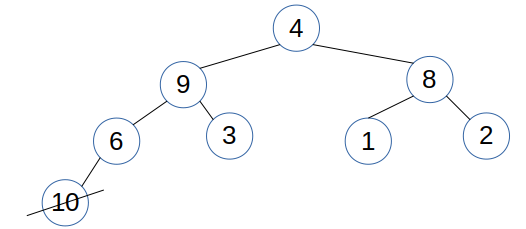
\includegraphics[scale=0.5]{./P16/r10}
\centering
\end{figure}


Now, reheap. From the bottom up, check if any elements are greater than their parents. 


\begin{figure}[H]
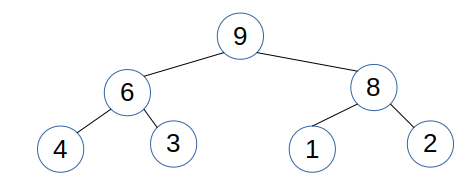
\includegraphics[scale=0.5]{./P16/m9}
\centering
\end{figure}

Swap max key with bottom right key, delete max key, reheap. Append this deleted key to the deleted list. 

\begin{figure}[H]
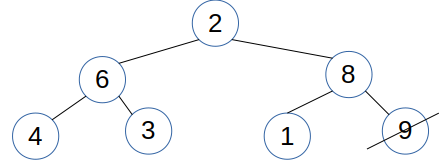
\includegraphics[scale=0.5]{./P16/r9}
\centering
\end{figure}

\begin{figure}[H]
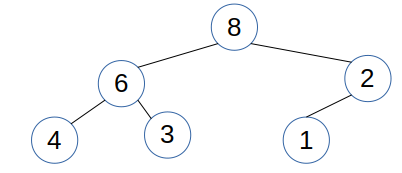
\includegraphics[scale=0.5]{./P16/m8}
\centering
\end{figure}

Same as before. 

\begin{figure}[H]
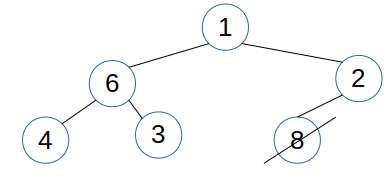
\includegraphics[scale=0.5]{./P16/r8}
\centering
\end{figure}

\begin{figure}[H]
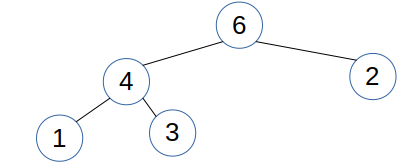
\includegraphics[scale=0.5]{./P16/m6}
\centering
\end{figure}

Same again. 

\begin{figure}[H]
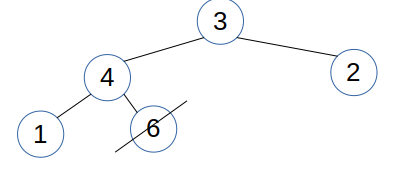
\includegraphics[scale=0.5]{./P16/r6}
\centering
\end{figure}


\begin{figure}[H]
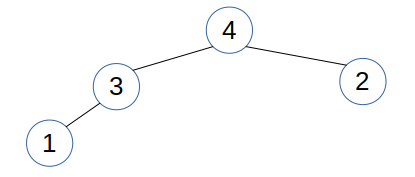
\includegraphics[scale=0.5]{./P16/m4}
\centering
\end{figure}

I'm getting tired. 

\begin{figure}[H]
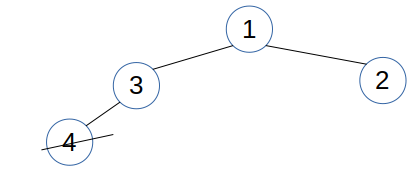
\includegraphics[scale=0.5]{./P16/r4}
\centering
\end{figure}

\begin{figure}[H]
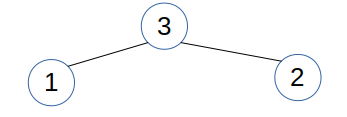
\includegraphics[scale=0.5]{./P16/m3}
\centering
\end{figure}

So close to done. 

\begin{figure}[H]
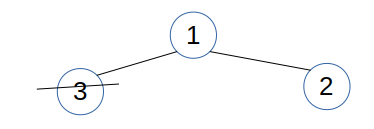
\includegraphics[scale=0.5]{./P16/r3}
\centering
\end{figure}

\begin{figure}[H]
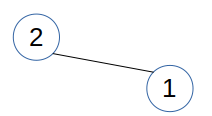
\includegraphics[scale=0.5]{./P16/m2}
\centering
\end{figure}

One more....

\begin{figure}[H]
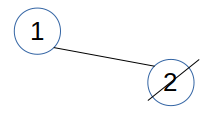
\includegraphics[scale=0.5]{./P16/r2}
\centering
\end{figure}


\begin{figure}[H]
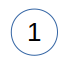
\includegraphics[scale=0.5]{./P16/m1}
\centering
\end{figure}

And we're done. 

Sorted list: 
1,2,3,4,6,8,9,10




\noindent\rule{8cm}{0.4pt}

17. 

\begin{lstlisting}
def quicksort(arr, left, right):
  if(left < right):
    print(arr) ###########
    pivot = partition(arr, left, right)
    print("^^Pivot = {}^^".format(arr[pivot])) ###########
    print()
    quicksort(arr, left, pivot - 1)
    quicksort(arr, pivot + 1, right)
  return arr

def partition(arr, left, right):
  pivot = left
  left += 1
  while True:
    #While l<=r and l hasn't reached pivot yet
    while left <= right and arr[left] < arr[pivot]:
        #Shift left to the right
      left += 1
    #While l<r and r hasn't reached pivot 
    while left <= right and arr[right] > arr[pivot]:
        #Shift right to the left
      right -= 1

    #If left and right did not cross, swap them and continue
    if left <= right:
      swap(arr, left, right)
      left += 1
      right -=1
    #Otherwise, break
    if left > right:
      break
  #Swap algorithm 
  swap(arr, right, pivot)
  return right

def swap(arr, a, b):
    c = arr[a]
    arr[a] = arr[b]
    arr[b] = c


def main():
    # Driver code to test above 
    arr = [9,8,7,6,5,4,3,2,1] 
    print("Original list: ")
    print(arr, sep=",")
    print()
    n = len(arr) 
    print("Implementing quicksort:")
    quicksort(arr,0,n-1) 
    print(arr,sep=",") 
    
if __name__ == '__main__':
    main()
\end{lstlisting}


\textbf{Output of quicksort}
As python does not have a good debugger that I know of for Linux, I implemented print statements in strategic places to check that the correct pivot was being chosen. The two lines in the quicksort() function with the inline comments after them print out the array and the partition selected on that recursion. 


\begin{lstlisting}
Original list: 
[9, 8, 7, 6, 5, 4, 3, 2, 1]

Implementing quicksort:
[9, 8, 7, 6, 5, 4, 3, 2, 1]
^^Pivot = 9^^

[1, 8, 7, 6, 5, 4, 3, 2, 9]
^^Pivot = 1^^

[1, 8, 7, 6, 5, 4, 3, 2, 9]
^^Pivot = 8^^

[1, 2, 7, 6, 5, 4, 3, 8, 9]
^^Pivot = 2^^

[1, 2, 7, 6, 5, 4, 3, 8, 9]
^^Pivot = 7^^

[1, 2, 3, 6, 5, 4, 7, 8, 9]
^^Pivot = 3^^

[1, 2, 3, 6, 5, 4, 7, 8, 9]
^^Pivot = 6^^

[1, 2, 3, 4, 5, 6, 7, 8, 9]
^^Pivot = 4^^

[1, 2, 3, 4, 5, 6, 7, 8, 9]

\end{lstlisting}


\textbf{MergeSort}

As with quicksort, I did not have an official debugger to use to check memory values. 
However, I did use a slight modification of merge sort to check which side of the array was being sorted. The character $s$ passed into the $mergesort()$ function tells the function whether it's sorting the left or the right side. As you can see in the output below, the program prints which side it's working on, and what the value of the array is at that point in the running of the program. 

\begin{lstlisting}
def mergeSort(arr,s=""): 
    _ = input("cont?")
    if len(arr) >1: 
        mid = len(arr)//2 #Using integer division
        L = arr[0:mid] # Dividing the array elements  
        R = arr[mid:len(arr)] # into 2 halves 
  
        #Recursively sort the arrays
        if(s=='r'):
            print("Sorting Right Side")
        print("Array value in this recursion: ", arr)
        mergeSort(R, 'r')
        print()

        if(s=='l'):
            print("Sorting Left Side")
        print("Array value in this recursion: ", arr)
        mergeSort(L, 'l')
        print()
  
        i = 0
        j = 0
        k = 0
          
        #Copy the first half of the array in L to the first half 
        #of the main array, and the second half of the array in R
        # to the second half of the main array.  
        while i < len(L) and j < len(R): 
            if L[i] < R[j]: 
                arr[k] = L[i] 
                i+=1
            else: 
                arr[k] = R[j] 
                j+=1
            k+=1
          
        #If any elements are left, fill them in automagically
        while i < len(L): 
            arr[k] = L[i] 
            i+=1
            k+=1
          
        while j < len(R): 
            arr[k] = R[j] 
            j+=1
            k+=1
  
# Code to print the list 
def printList(arr): 
    for i in range(len(arr)):         
        print(arr[i],end=" ") 
    print() 
  
def main():
    arr = [1,5,3,9,7,12,15,45,96]  
    print ("Given array is", end="\n")  
    printList(arr) 
    mergeSort(arr) 
    print("Sorted array is: ", end="\n") 
    printList(arr) 

if __name__ == '__main__':
    main()

\end{lstlisting}

\begin{lstlisting}
Given array is
1 5 3 9 7 12 15 45 96 
cont?
Array value in this recursion:  [1, 5, 3, 9, 7, 12, 15, 45, 96]
cont?
Sorting Right Side
Array value in this recursion:  [7, 12, 15, 45, 96]
cont?
Sorting Right Side
Array value in this recursion:  [15, 45, 96]
cont?
Sorting Right Side
Array value in this recursion:  [45, 96]
cont?

Array value in this recursion:  [45, 96]
cont?


Array value in this recursion:  [15, 45, 96]
cont?


Array value in this recursion:  [7, 12, 15, 45, 96]
cont?
Array value in this recursion:  [7, 12]
cont?

Sorting Left Side
Array value in this recursion:  [7, 12]
cont?



Array value in this recursion:  [1, 5, 3, 9, 7, 12, 15, 45, 96]
cont?
Array value in this recursion:  [1, 5, 3, 9]
cont?
Sorting Right Side
Array value in this recursion:  [3, 9]
cont?

Array value in this recursion:  [3, 9]
cont?


Sorting Left Side
Array value in this recursion:  [1, 5, 3, 9]
cont?
Array value in this recursion:  [1, 5]
cont?

Sorting Left Side
Array value in this recursion:  [1, 5]
cont?



Sorted array is: 
1 3 5 7 9 12 15 45 96 
\end{lstlisting}



\noindent\rule{8cm}{0.4pt}


18. 

\textbf{Depth first algorithm}

\begin{lstlisting}
def dfs(graph, start, visited=None, round=0):

    #If no nodes have been visited, create 
    # an empty set for adding. 
    if visited is None:
        print("No nodes visited. Creating empty list. ")
        visited = set()

    # Add the starting node for this recursion
    # to the visited stack
    visited.add(start)

    #Increment a round counter
    round += 1
    print("\n--->Round {}<---".format(round))

    #Print out the visited nodes.
    print("Nodes visited -->{}<--".format(visited))

    print("Visiting {}.".format(start))
    for next in graph[start] - visited:
        print("Checking node {}".format(next))

        #Recursively continue through graph
        #Code referenced from https://www.programiz.com/dsa/graph-dfs
        dfs(graph, next, visited, round)
    return visited

def getInput():

    graph = {}

    num = int(input("Enter the number of nodes in the graph >> "))

    for i in range(num):

        i = str(i)

        key = []

        line = input("Enter the nodes attached to node {}>> ".format(i))

        for number in line:
            if number.isdigit():
                key.append(number)

        graph[i] = set(key)


    return graph

def main():
    dfs(getInput(), '0')
if __name__ == '__main__':
    main()
\end{lstlisting}

\textbf{Output of BFS:}

\begin{lstlisting}
Enter the number of nodes in the graph >> 7
Enter the nodes attached to node 0>> 1,2
Enter the nodes attached to node 1>> 0,3,4
Enter the nodes attached to node 2>> 0,5,6
Enter the nodes attached to node 3>> 1
Enter the nodes attached to node 4>> 1
Enter the nodes attached to node 5>> 2
Enter the nodes attached to node 6>> 2
No nodes visited. Creating empty list. 

--->Round 1<---
Nodes visited -->{'0'}<--
Visiting 0.
Checking node 2

--->Round 2<---
Nodes visited -->{'2', '0'}<--
Visiting 2.
Checking node 5

--->Round 3<---
Nodes visited -->{'2', '0', '5'}<--
Visiting 5.
Checking node 6

--->Round 3<---
Nodes visited -->{'2', '0', '5', '6'}<--
Visiting 6.
Checking node 1

--->Round 2<---
Nodes visited -->{'6', '5', '2', '0', '1'}<--
Visiting 1.
Checking node 4

--->Round 3<---
Nodes visited -->{'6', '4', '5', '2', '0', '1'}<--
Visiting 4.
Checking node 3

--->Round 3<---
Nodes visited -->{'6', '4', '5', '2', '0', '3', '1'}<--
Visiting 3.


\end{lstlisting}


\textbf{Breadth First Search}
\begin{lstlisting}
import collections

#Define the bfs algorithm
def bfs(g, rootnode):

    #Use set() to create an empty set
    #This is the set of visited nodes, which 
    # we will add to as we progress through 
    # the graph
    visited = set()

    #Dequeue the first element in the list
    queue = collections.deque([rootnode])

    #Now that the root node has been dequeued,
    # add it to the visited set. We will not visit
    # this node again. 
    visited.add(rootnode)

    #Use a counter to keep track of rounds
    round = 0

    while queue: 
        print("\nRound {}".format(round))

        #Dequeue the first element in the list. 
        vertex = queue.popleft()
        print("Popped vertex {} from queue".format(vertex))


        #Find each neighbor for the vertex
        for neighbor in g[vertex]: 
            print("Checking neighbor {}".format(neighbor))
            if neighbor not in visited: 
                print("Visiting node {0} on round {1}".format(neighbor, round))

                #Now that it has been visited, add the
                # neighbor to the visisted set. 
                visited.add(neighbor) 

                #Also, queue the neighbor 
                # to be visited in a future round. 
                queue.append(neighbor) 
            else:
                print("Node {0} has already been visited.".format(neighbor))
        #Increment the counter. 
        round += 1

def getInput():
    graph = {}
    num = int(input("Enter the number of nodes in the graph >> "))
    for i in range(num):
        key = []

        line = input("Enter the nodes attached to node {}>> ".format(i))
        for number in line:
            if number.isdigit():
                key.append(int(number))
        graph[i] = key
    return graph

def main():
    bfs(getInput(), 0)


if __name__ == '__main__':
    main()
\end{lstlisting}


\textbf{Output of BFS}
\begin{lstlisting}
Enter the number of nodes in the graph >> 7
Enter the nodes attached to node 0>> 1,2
Enter the nodes attached to node 1>> 0,3,4
Enter the nodes attached to node 2>> 0,5,6
Enter the nodes attached to node 3>> 1   
Enter the nodes attached to node 4>> 1
Enter the nodes attached to node 5>> 2
Enter the nodes attached to node 6>> 2

Round 0
Popped vertex 0 from queue
Checking neighbor 1
Visiting node 1 on round 0
Checking neighbor 2
Visiting node 2 on round 0

Round 1
Popped vertex 1 from queue
Checking neighbor 0
Node 0 has already been visited.
Checking neighbor 3
Visiting node 3 on round 1
Checking neighbor 4
Visiting node 4 on round 1

Round 2
Popped vertex 2 from queue
Checking neighbor 0
Node 0 has already been visited.
Checking neighbor 5
Visiting node 5 on round 2
Checking neighbor 6
Visiting node 6 on round 2

Round 3
Popped vertex 3 from queue
Checking neighbor 1
Node 1 has already been visited.

Round 4
Popped vertex 4 from queue
Checking neighbor 1
Node 1 has already been visited.

Round 5
Popped vertex 5 from queue
Checking neighbor 2
Node 2 has already been visited.

Round 6
Popped vertex 6 from queue
Checking neighbor 2
Node 2 has already been visited.

\end{lstlisting}

\noindent\rule{8cm}{0.4pt}

\end{document}
